%%%%%%%%%%%%%%%%%%%%%%%%%%%%%%%%%%%%%%%%%%%%%%%%%%%%%%%%%%%%%%%%%%%%%%%%
% Escuela Politécnica Superior de la Universidad de Alicante
% Realizado por: Jose Manuel Requena Plens
% Contacto: info@jmrplens.com / Telegram:@jmrplens
%%%%%%%%%%%%%%%%%%%%%%%%%%%%%%%%%%%%%%%%%%%%%%%%%%%%%%%%%%%%%%%%%%%%%%%%

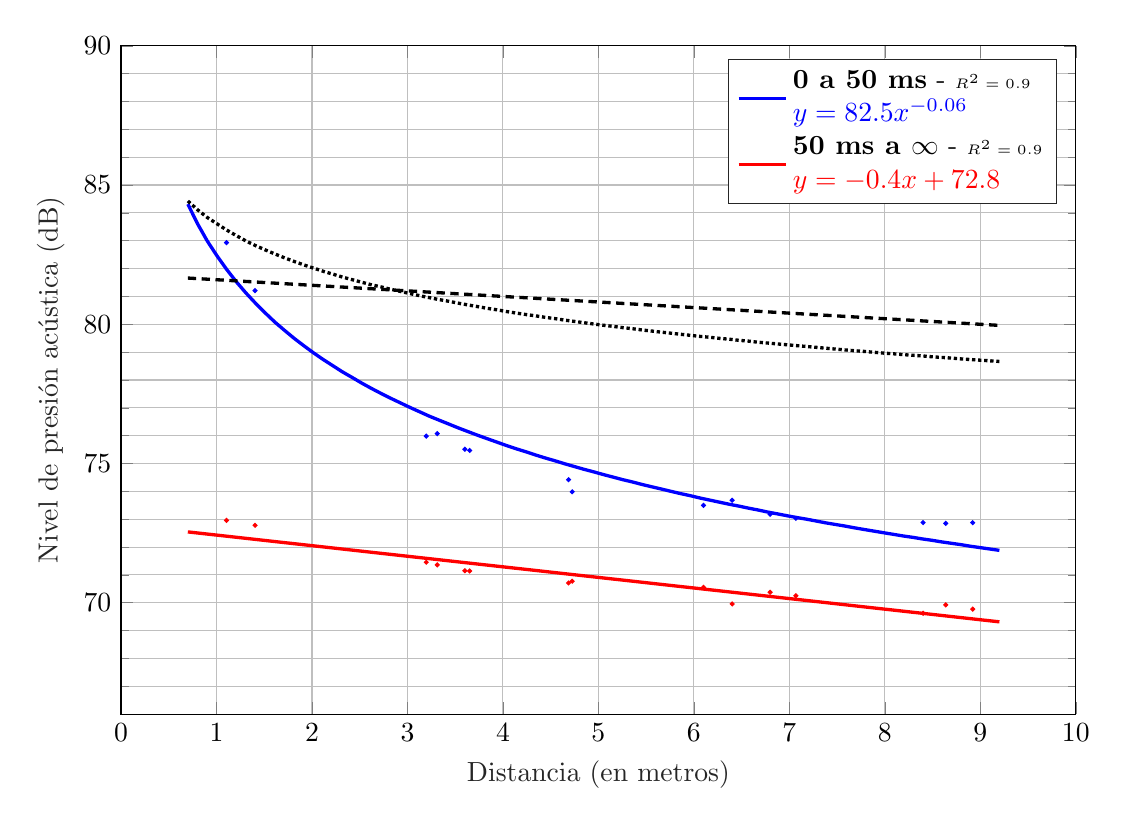
\begin{tikzpicture}

\begin{axis}[%
width=\textwidth,
height=0.7\textwidth,
at={(0\textwidth,0\textwidth)},
scale only axis,
xmin=0,
xmax=10,
xlabel style={font=\color{white!15!black}},
xlabel={Distancia (en metros)},
ymin=66,
ymax=90,
ylabel style={font=\color{white!15!black}},
ylabel={Nivel de presión acústica (dB)},
axis background/.style={fill=white},
xmajorgrids,
xminorgrids,
ymajorgrids,
yminorgrids,
minor y tick num= 4,
legend style={legend cell align=left, align=left, draw=white!15!black}
]
% Curvas CATT
\addplot[color=blue,domain=0.7:9.2, samples=85,line width=1.2]{82.47*x^(-0.062)};
\addlegendentry{\textbf{0 a 50 ms} - \tiny{$R^2 = 0.9$}\\$\color{blue}y = 82.5·x^{-0.06}$}

\addplot[color=red,domain=0.7:9.2, samples=85,line width=1.2]{-0.38*x+72.81};
\addlegendentry{\textbf{50 ms a $\infty$} - \tiny{$R^2 = 0.9$}\\$\color{red}y = -0.4·x+72.8$}

% Curvas in situ
\addplot[color=black,densely dotted,line width=1.2pt,domain=0.7:9.2, samples=85]{76.9*x^(-0.03)+6.7};
\addplot[color=black,densely dashed,line width=1.2pt,domain=0.7:9.2, samples=85]{-0.2*x+75.1+6.7};

% Puntos
\addplot [color=blue, only marks,mark size=0.7pt]
  table[row sep=crcr]{%
  1.10453610171873	82.9345303709531\\
1.40356688476182	81.2102515329224\\
3.19687347262916	75.9856271063767\\
3.31209903233584	76.0756440395286\\
3.60138862107382	75.5150762506015\\
3.65136960605195	75.4708681827389\\
4.68721665810319	74.4180957656198\\
4.72572745722815	73.9855579847906\\
6.10081961706786	73.4964261025427\\
6.40078120232210	73.6785459543595\\
6.79852925271341	73.1772931521972\\
7.06894617322837	73.0315844338110\\
8.40059521700695	72.8777411592766\\
8.63828686719769	72.8483022158284\\
8.92020179143947	72.8746507896277\\
  };
  
  \addplot [color=red, only marks,mark size=0.7pt]
  table[row sep=crcr]{%
  1.10453610171873	72.9562307280560\\
1.40356688476182	72.7819124497572\\
3.19687347262916	71.4545090236686\\
3.31209903233584	71.3575091767311\\
3.60138862107382	71.1480243215088\\
3.65136960605195	71.1422849661127\\
4.68721665810319	70.7100903981730\\
4.72572745722815	70.7730643726906\\
6.10081961706786	70.5520001586585\\
6.40078120232210	69.9591314519951\\
6.79852925271341	70.3752685657530\\
7.06894617322837	70.2508837688623\\
8.40059521700695	69.6209970304835\\
8.63828686719769	69.9245634923070\\
8.92020179143947	69.7722037094251\\
  };
\end{axis}
\end{tikzpicture}%